\documentclass[tikz]{standalone}
\usepackage{calc}
\usepackage{tikz}
\usetikzlibrary{matrix,fit,backgrounds,calc,decorations.markings,arrows.meta,shapes.geometric,tikzmark,math}
\usepackage{amsmath}
\usepackage{braket}

\begin{document}
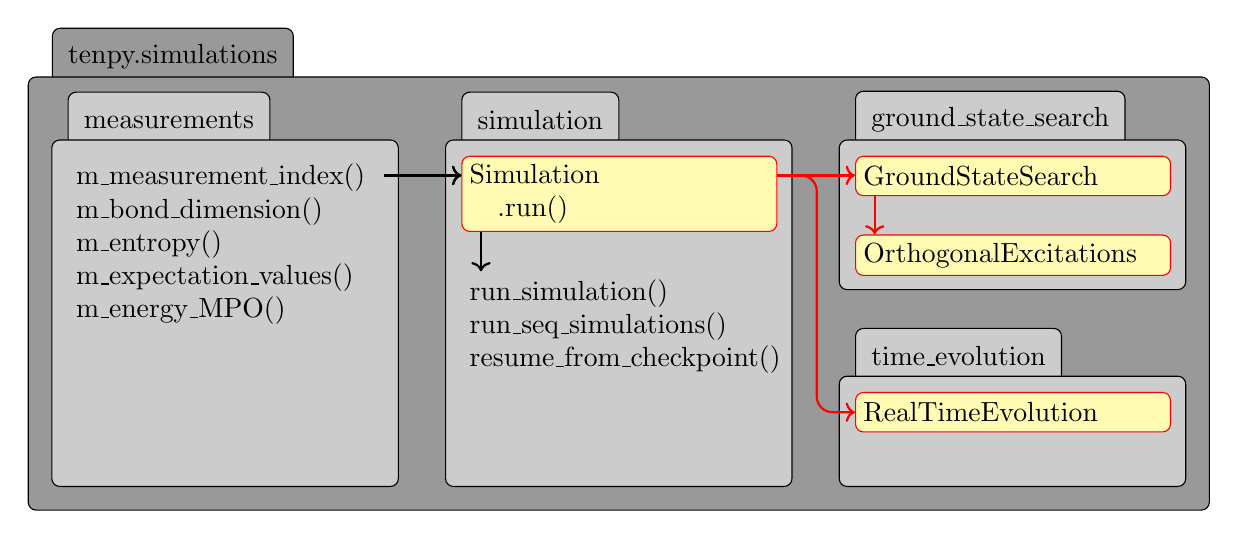
\begin{tikzpicture}[
		remember picture,
		modulecontent/.style={rounded corners=1mm,inner sep=1mm,node font=\texttt,
			minimum height=0.5cm,text width=3.8cm,anchor=north west},
		class/.style={modulecontent,draw=red,fill=yellow!30},
		subclass/.style={class=#1,text width=3.3cm},
		used_in/.style={thick,rounded corners=2mm},
		inherit/.style={thick,color=red,rounded corners=2mm},
		%
		package/.style={draw,fill=black!40,rounded corners=1mm,inner sep=2mm},
		subpackage/.style={draw,fill=black!20,rounded corners=1mm,inner sep=2mm},
		pics/package/.style n args={2}{code={
			\node[package,anchor=south west,minimum height=7mm] at (-2mm,9mm) {#1};
			\path[package] (-5mm,10mm)  rectangle ($ #2 + (5mm,-5mm)$) ;
		}},
		pics/subpackage/.style n args={2}{code={
			\node[subpackage,anchor=south west,minimum height=7mm] at (0,1mm) {#1};
			\path[subpackage] (-2mm,2mm)  rectangle ($ #2 + (2mm,-2mm)$) ;
		}}%
	]
	\tikzmath{\colw=5; \classw=4; \subind=0.5;
		%\cb{n} = class begin{n}; \cs{n} = subclass begin; \ce{n} = class end
		\cb1 = 1*\colw - \colw; \cs1 = \cb1 + \subind; \ce1 = \cb1 + \classw ;
		\cb2 = 2*\colw - \colw; \cs2 = \cb2 + \subind; \ce2 = \cb2 + \classw ;
		\cb3 = 3*\colw - \colw; \cs3 = \cb3 + \subind; \ce3 = \cb3 + \classw ;
	}
	%
	\begin{scope}[xshift=0cm,yshift=0cm]
		\draw pic at (\cb1, 0) {package={tenpy.simulations}{(\ce3,-4)}};
		\draw pic at (\cb1, 0) {subpackage={measurements}{(\ce1,-4)}};
		\draw pic at (\cb2, 0) {subpackage={simulation}{(\ce1,-4)}};
		\draw pic at (\cb3, 0) {subpackage={ground\_state\_search}{(\ce1,-1.5)}};
		\draw pic at (\cb3, -3) {subpackage={time\_evolution}{(\ce1,-1)}};
		\node[modulecontent] (meas_fct)   at (\cb1, 0) {
			m\_measurement\_index() \\
			m\_bond\_dimension() \\
			m\_entropy() \\
			m\_expectation\_values() \\
			m\_energy\_MPO() 
		};
		\node[class]         (Simulation) at (\cb2, 0) {Simulation \\
			\quad .run()  \\
			% \quad .init\_model()  \\
			% \quad .init\_state() \\
			% \quad .init\_measurements()\\
			% \quad .save\_results()
			};
		\node[modulecontent] (sim_fct)    at ($ (Simulation.south west) + (0,-0.5) $) {%
				run\_simulation()  \\
				run\_seq\_simulations()  \\
				resume\_from\_checkpoint()
			};
		\node[class]         (GroundStateSearch) at (\cb3, 0) {GroundStateSearch};
		\node[class]         (Ortho) at (\cb3,-1) {OrthogonalExcitations};
		\node[class]         (RealTimeEvolution) at (\cb3,-3) {RealTimeEvolution};
		%
		\draw[inherit,->] ($ (Simulation.north east) + (0,-0.25) $) --  ($ (GroundStateSearch.north west) + (0,-0.25) $);
			\draw[inherit,->] ($ (Simulation.north east) + (0,-0.25) $) -- +(0.5,0) |- (RealTimeEvolution.west) ;
		\draw[inherit,->] ($ (GroundStateSearch.south west) + (0.25,0) $) --  ($ (Ortho.north west) + (0.25,0) $);
		\draw[used_in,->] ($ (meas_fct.north east) + (0,-0.25) $) --  ($ (Simulation.north west) + (0,-0.25) $);
		\draw[used_in,->] ($ (meas_fct.north east) + (0,-0.25) $) --  ($ (Simulation.north west) + (0,-0.25) $);
		\draw[used_in,->] ($ (Simulation.south west) + (0.25, 0) $) --  ($ (sim_fct.north west) + (0.25,0) $);
		% \foreach \src in {LegCharge,LegPipe}
		%     \draw[used_in,->] (\src.east) -- +(0.5,0) |- ($ (Array.west) + (0,0.3) $);
		% \draw[used_in,->] ($ (Array.south west) + (1,0) $) --  ($ (npc_fct.north west) + (1,0) $);
		% \draw[used_in,->] ($ (Array.north east) + (0,-0.25) $) --  ($ (KrylovBased.north west) + (0,-0.25) $);
		% \foreach \subcls in {Arnoldi,LanczosGroundState,LanczosEvolution}
		%     \draw[inherit,->] ($ (KrylovBased.south west) + (0.2,0) $) |- (\subcls.west) ;
	\end{scope}
	% coordinates
	% \draw[very thin, color=blue] (-2.0,-5.0) grid (5.0,3.0);
	% \draw[thick,color=blue,->] (-2.,0) -- (5., 0.) ;
	% \draw[thick,color=blue,->] (0., -5.) -- (0., 5) ;
	% \foreach \i in {-3,...,5}
	% {
	%     \node at (0,\i) {\i{}};
	%     \node at (\i,0) {\i{}};
	% }
\end{tikzpicture}
\end{document}
